
\minitoc%

\section{Pourquoi viser l'estimation des couples d'incréments plutôt que la régularité}
\label{annexe:choix_risque_couple}

\info{
	on rappelle les notations suivantes :

	\begin{itemize}
		\item vrai : $\theta = \mathds E \bigl[ \, f(X) \, \bigr]$
		\item intangible/inobservable : $\widetilde \theta = \frac 1 N \sum_i f(X_i)$
		\item observable : $\widehat \theta = \frac 1 N \sum_i f(\widehat X_i)$
	\end{itemize}
}

L'estimation des paramètres de régularité locale en $t_2$, $H_{t_2}$ et $L_{t_2}$, utilise les incréments quadratiques $\theta$ entre les différents points $t_1, t_2, t_3$ situés dans un voisinage de diamètre $\Delta$ autour de $t_2$.

\question{
	Quelle quantité est-il judicieux d'évaluer pour estimer au mieux la régularité locale en $t_2$ ? Doit-t-on regarder la qualité de l'approximation de $\theta$ (qui est une espérance) car il est utilisé pour tous les estimateurs ? Ou doit-on regarder la qualité de l'approximation de $H_{t_2}$ et $L_{t_2}$ car ce sont les quantités qui nous intéressent ? Ou bien les deux ?
}

Le choix du bon critère d'évaluation est d'une grande importance. Il faut se rappeler l'objectif que l'on cherche à atteindre : déterminer une procédure (simple si possible) de détermination de l'hyper-paramètre $\Delta$ utilisé pour l'estimation de la régularité locale en fonction de quantités facilement estimables, ou directement observables par le praticien. En observant que $L$ est estimée par une expression impliquant $\theta$ et $\Delta^{2 H}$, une estimation précise de $H$ paraît plus cruciale pour la bonne estimation des deux quantités. Bien qu'il existe certainement un compromis entre la bonne estimation de $H$ et de $L$ qui fournit une meilleure estimation adaptative des quantités qui nous intéressent, il est certainement plus probable de dériver une procédure de sélection de $\Delta$ simple à implémenter pour le praticien en se basant sur la qualité de l'estimation d'une unique quantité.

\question{
	Doit-t-on se concentrer sur l'estimation de $H$ ou de $\theta$ ?
}

Les incréments sont des quantités importantes dans l'estimation de la régularité, utilisées à la fois pour l'estimation de $H$ et de $L$, l'approche que l'on considère se base sur cette remarque. Nous allons donc chercher à déterminer un $\Delta$ adapté à l'estimation des incréments quadratiques. Toutefois, il y a plusieurs possibilités de $u,v \in J_\Delta(t_2)$ que l'on peut considérer pour l'estimation de $H$ et $L$. C'est pourquoi nous décidons de considérer les \emph{couples} d'incréments utilisés pour l'estimation de $H$. Ainsi en posant :

\begin{minipage}{0.5\textwidth}
	\begin{equation*}
		\thetaA = \begin{bmatrix} \theta(t_1, t_3) \\ \theta(t_1, t_2) \end{bmatrix}
	\end{equation*}
\end{minipage}
\hfill
\begin{minipage}{0.5\textwidth}
	\begin{equation*}
		\thetaB = \begin{bmatrix} \theta(t_1, t_3) \\ \theta(t_2, t_3) \end{bmatrix}
	\end{equation*}
\end{minipage}

\smallskip

L'estimateur du paramètre de régularité $H_t$ peut se ré-écrire comme :

\smallskip


\begin{equation*}
	\widehat H_t : \Theta = \begin{bmatrix} \Theta_1 \\ \Theta_2 \end{bmatrix} \longmapsto \frac{ \log \widehat \Theta_1 - \log \widehat \Theta_2 }{2 \log 2}
\end{equation*}

\smallskip

Le problème c'est qu'on ne dispose pas de la véritable valeur de $\theta(u,v)$, on pourrait exploiter le fait que l'on dipose d'un mouvement brownien multi-fractionnaire qui a été étudié de façon extensive dans la littérature, mais on décide de ne pas l'utiliser pour adopter une approche plus proche d'un cadre général.
Le meilleur estimateur que l'on puisse espérer atteindre est l'estimateur de l'espérance par la moyenne empirique des courbes non bruitées :
 
\begin{equation*}
\widetilde H_t( \thetaA) \quad \textsf{ou} \quad \widetilde H_t(  \thetaB)
\end{equation*}

avec $\widetilde H_t : \Theta \mapsto \frac{ \log \widetilde\Theta_1 - \log \widetilde\Theta_2 }{2 \log 2}$

\bigskip

\noindent On va donc s'intéresser désormais à l'erreur d'estimation conjointe des deux $\theta(u,v)$ utilisés dans l'estimation de $H_t$ par rapport à cet estimateur en quelque sorte \og idéal \fg de $\theta$ comme critère de sélection du diamètre $\Delta$.

\begin{figure}[H]
	\centering
	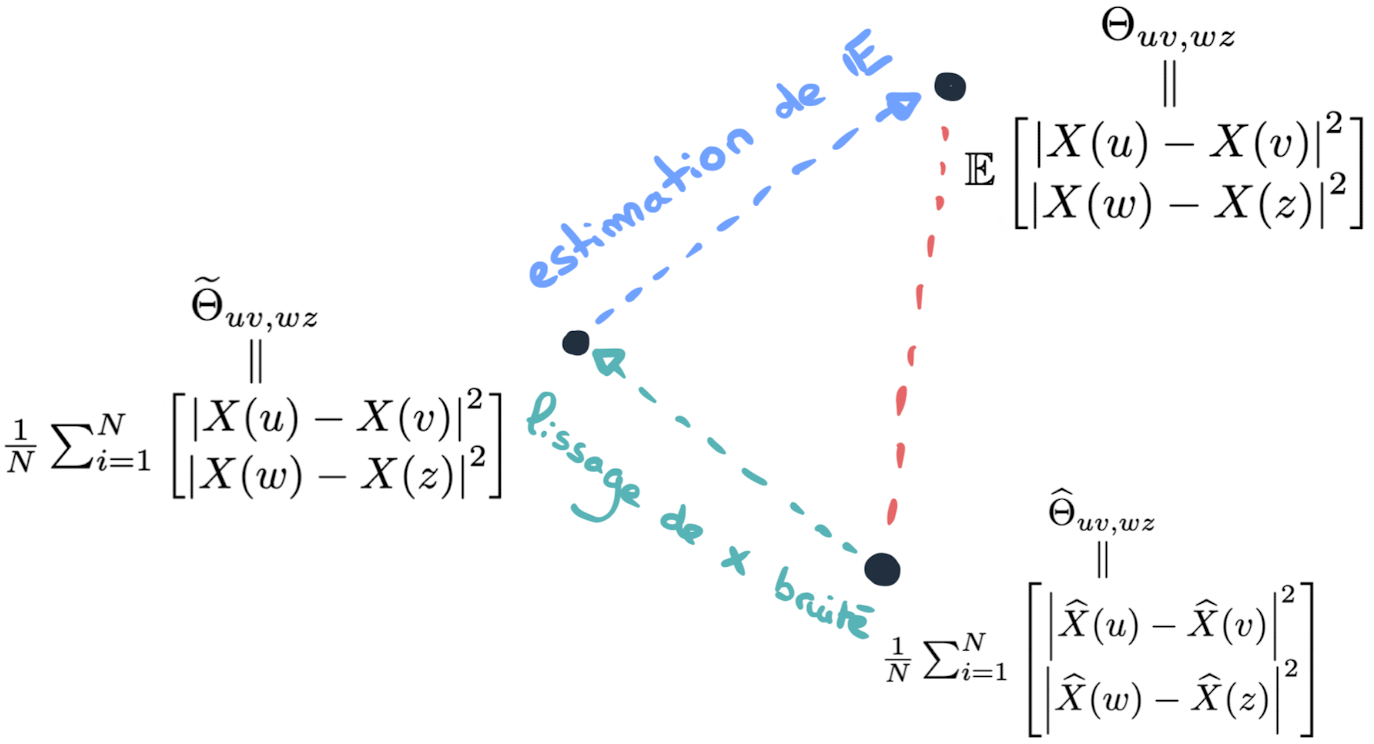
\includegraphics[width=0.7\textwidth]{Images/sketches/theta_biais.png}
	\caption{Schéma représentant les différentes approximations du couple d'incréments}
	\label{fig:sketch_theta_biais}
\end{figure}

\subsection{Choix du Risque}

\subsubsection{Distance Euclidienne}

Afin de quantifier la qualité de l'estimation conjointe du couple de $\theta$, il est raisonnable de considérer la distance euclidienne usuelle pour des vecteurs de $\R 2$

\begin{equation*}
R(\Theta, \Delta) = {\distnorme 2 {\widehat \Theta(\Delta)} {\widetilde \Theta(\Delta)}}^2
\end{equation*}

% et on nomme $R\cindexA(\Delta) = R( \thetaA , \, \Delta \, )$ et $R\cindexB(\Delta) = R( \thetaB, \, \Delta \, )$

\subsubsection{Distance Euclidienne Relative}

On va cependant considérer le risque relatif à la norme de la quantité que l'on cible :

\begin{equation*}
R(\Theta, \Delta) =\frac{ {\distnorme 2 {\widehat \Theta(\Delta)} {\widetilde \Theta(\Delta)}}^2}{ {\norme 2 {\widetilde \Theta(\Delta)}}^2 }
\end{equation*}

\question{Pourquoi considérer la distance euclidienne relative à la norme de la cible $\widetilde \Theta$ plutôt que la distance euclidienne classique qui est plus simple ?}

Le risque sert à déterminer la qualité de l'estimation du couple $\widetilde \Theta$ par $\widehat \Theta$ à un $\Delta$ donné. Il faut cependant garder à l'esprit que $\Theta$ est en réalité une fonction de $\Delta$ car la valeur de $t_1, t_2, t_3$ dépendent de $\Delta$. Ainsi la norme de $\widetilde \Theta$ va varier lorsque l'on fait varier $\Delta$\footnote{il est possible d'obtenir plus de détails en annexe \ref{annexe:tous_theta_conviennent_borne_norme_theta}}. Les risques obtenus via la norme euclidienne sont des risques qui mesurent une différence absolue, mais alors avoir un risque plus petit qu'un autre n'a pas le même sens pour différents $\Delta$ en termes de qualité d'approximation. C'est pourquoi nous considérons le risque relatif dans la détermination du critère du choix du $\Delta$.

On pourra cependant observer la différence entre le risque euclidien et le risque euclidien relatif à la norme de la cible en $\Delta$ sur les figures \ref{fig:sparse_osef} et \ref{fig:sparse_osef_rel}.

\section[Peut-on considérer que tous les delta conviennent ?]{Peut-on considérer que tous les $\Delta$ conviennent ?}
\label{annexe:tous_theta_conviennent_borne_norme_theta}
Nous considérons le risque euclidien : $\mathcal R(\Theta, \Delta) = \mathds E \distnorme 2 {\widehat \Theta}{\widetilde \Theta}$. C'est un risque naturel à considérer pour une estimation conjointe de deux paramètres. Evidemment, nous ne disposons pas de la loi de $\distnorme 2 {\widehat \Theta}{\widetilde \Theta}$ c'est pourquoi nous calculons $\widehat {\mathcal R}(\Theta, \Delta) = \mathds E \distnorme 2 {\widehat \Theta}{\widetilde \Theta}$

Nous observons sur les différents graphes des risques de l'ordre de grandeur de $10^{-2}$ ou même de $10^{-3}$. La question que l'on se pose désormais est si il est raisonnable de penser que ne pas choisir le $\Delta^*$ optimal n'est pas si important dans l'estimation du couple $\Theta$.

Ce que nous allons observer est qu'il est tout de même préférable de bien déterminer le $\Delta$

\begin{equation}
	\theta(u,v) = \esperanceloi X { \bigl| X(v) - X(u) \bigr|^2 } \leq L_{J(\Delta)}^2 \bigl| v - u \bigr|^{2 H_{J(\Delta)}}
\end{equation}

sachant que l'on évalue :

\begin{equation}
	\textsf{soit }
	\thetaA = \begin{bmatrix} \theta(t_1, t_3) \\ \theta(t_1, t_2) \end{bmatrix}
\end{equation}
\begin{equation}
	\textsf{soit }
	\thetaB = \begin{bmatrix} \theta(t_1, t_3) \\ \theta(t_2, t_3) \end{bmatrix}
\end{equation}


avec :

\begin{equation}
	\begin{array}{ccc}
		|t_3 - t_1| & = \Delta
		\\
		|t_3 - t_2| & = \frac \Delta 2 & = |t_2 - t_1|
	\end{array}\label{eq:couples_diff_delta_value}
\end{equation}

et donc :

\begin{equation}
	\displaystyle
	\begin{array}{rclr}
		\norme 2 \Theta & =    & \sqrt{\theta_{13}^{\,2} + \theta_{12/23}^{\, 2}}
		\\
		                & \leq & \sqrt{ L_{J(\Delta)}^4 \bigl( \, \Delta^{4 H_{J(\Delta)}} \left[ 1 + \frac 1 2 \right]  \, \bigr) }
		\\
		                & =    & L_{J(\Delta)}^2 \cdot \Delta^{2H_{J(\Delta)}} \cdot \sqrt{\frac 3 2}
	\end{array}
\end{equation}

Et donc :

\begin{equation*}
	\norme 2 \Theta \leq L_{J(\Delta)}^2 \cdot \Delta^{2H_{J(\Delta)}} \cdot \sqrt{\frac 3 2}
\end{equation*}

On se réfère à ces bornes même si l'on étudie plutôt $\widetilde \Theta$ car on peut se ramener asymptotiquement à $\Theta$ par la loi des grands nombres grâce à la dépendance faible :

\begin{align}
	 &  & \norme 2 {\widetilde \Theta} & =                                                                                                                      & \norme 2 {\frac 1 N \sum_{i=1}^{N} \begin{bmatrix} | X_i(t_3) - X_i(t_1) |^2 \\ | X_i(t_3) - X_i(t_2) |^2 \end{bmatrix}} &  &
	\\
	 &  &                              & \overset {\textsf{LGN} + \textsf{dep. faible} + \textsf{norme } \mathcal C^0(\R 2) }{\tend N \infty } & \norme 2 \Theta \leq L_{J(\Delta)}^2 \cdot \Delta^{2H_{J(\Delta)}} \cdot \sqrt{\frac 3 2}                                &  &
\end{align}

\begin{rem}
	On peut remplacer le couple $(t_2, t_3)$ par $(t_1, t_2)$ dans la deuxième composante, l'argument reste valide, comme explicité dans l'équation \ref{eq:couples_diff_delta_value}
\end{rem}

En utilisant les données de la simulation, $L = 1$, on obtient :

\begin{equation}
	\begin{array}{ccc}
		H_{J(\Delta)} = 0.4  & \implies & \norme 2 \Theta
		\begin{cases}
			\lesssim 3 \cdot 10^{-2} \quad & \Delta = 0.01
			\\
			\lesssim 3\cdot 10^{-1} \quad  & \Delta = 0.2
		\end{cases}
		\\\\
		H_{J(\Delta)} = 0.5  & \implies & \norme 2 \Theta
		\begin{cases}
			\lesssim 1 \cdot 10^{-2} \quad & \Delta = 0.01
			\\
			\lesssim 2\cdot 10^{-1} \quad  & \Delta = 0.2
		\end{cases}
		\\\\
		H_{J(\Delta)} = 0.6  & \implies & \norme 2 \Theta
		\begin{cases}
			\lesssim 5 \cdot 10^{-3} \quad & \Delta = 0.01
			\\
			\lesssim 2\cdot 10^{-1} \quad  & \Delta = 0.2
		\end{cases}
		\\\\
		H_{J(\Delta)} = 0.73 & \implies & \norme 2 \Theta
		\begin{cases}
			\lesssim 1 \cdot 10^{-3} \quad & \Delta = 0.01
			\\
			\lesssim 1\cdot 10^{-1} \quad  & \Delta = 0.2
		\end{cases}
	\end{array}
\end{equation}

Ainsi, la différence de risque entre l'optimum et le pire cas étant de l'odre de $10^{-2}$ dans un cas très sparse comme dans la figure \ref{fig:sparse_osef} et dans un cas raisonnablement dense on observe même des différences de l'ordre de $10^{-3}$ pour le plus régulier.

\begin{table}[H]
	\centering
	\begin{tabularx}{0.7\textwidth}{|cc|X|X|c|}
		\toprule
		\textbf{H} & $\mathbf{\lambda}$ & \textbf{Différence : } $\mathbf{\mathcal R_{max} - \mathcal R_{min}}$ & ordre de gradeur de la borne de $\norme 2 \Theta$ & ${\norme 2 \Theta}^2$ \\
		\midrule
		0.51       & 60                 & 3.3 $\cdot 10^{-2}$                                                   & $\Delta^* \simeq 0.2$ : $10^{-1}$                 & $10^{-2}$             \\
		0.51       & 210                & 1.1 $\cdot 10^{-2}$                                                   & $\Delta^* \simeq 0.2$ : $10^{-1}$                 & $10^{-2}$             \\
		\midrule
		0.6        & 60                 & 4.2 $\cdot 10^{-2}$                                                   & $\Delta^* \simeq 0.01$ : $10^{-3}$                & $10^{-6}$             \\
		0.6        & 210                & 1.2 $\cdot 10^{-2}$                                                   & $\Delta^* \simeq 0.01$ : $10^{-3}$                & $10^{-6}$             \\
		\midrule
		0.73       & 60                 & 1.2 $\cdot 10^{-2}$                                                   & $\Delta^* \simeq 0.01$ : $10^{-3}$                & $10^{-6}$             \\
		0.73       & 210                & 5.4 $\cdot 10^{-3}$                                                   & $\Delta^* \simeq 0.01$ : $10^{-3}$                & $10^{-6}$             \\
		\bottomrule
	\end{tabularx}
	\caption{Ordre de grandeur des différences entre le risque euclidien minimum et maximum pour $\Delta \in [0.01, 0.2]$ et la norme de la cible}
	\label{tab:ordre_grandeur_diff_R_norme}
	\addcontentsline{lot}{table}{\numberline{} Comparaison des ordres de grandeur de la norme de la quantité ciblée $\widetilde \Theta$ et de différence entre le risque optimal et maximal.}
\end{table}

\noindent Étant donné que le risque utilisé est homogène à la norme euclidienne au carré, on ne peut dire, du point de vue du risque euclidien, que l'on peut prendre n'importe quel $\Delta$ dans $[0.01, 0.2]$ sans trop de conséquences.
Ce tableau vient motiver la section suivante sur le choix du risque à considérer pour la détermination d'un $\Delta$ optimal. Si la norme de notre cible varie avec $\Delta$, une idée est de plutôt considérer la qualité de l'estimation, relativement à la norme de la cible.


\section{Choix du risque : absolu ou relatif ?}
\label{annexe:choix-du-rique}
\subsection{Distance Euclidienne}

Afin de quantifier la qualité de l'estimation conjointe du couple de $\theta$, il est raisonnable de considérer la distance euclidienne usuelle pour des vecteurs de $\R 2$

\begin{equation*}
	R^{[\,rel\,]}_{mc}(\Theta, \Delta) = {\distnorme 2 {\widehat \Theta(\Delta)} {\widetilde \Theta(\Delta)}}^2
\end{equation*}

\subsection{Distance Euclidienne Relative}

On va cependant considérer le risque relatif à la norme de la quantité que l'on cible :

\begin{equation*}
	R^{[\,rel\,]}_{mc}(\Theta, \Delta) =\frac{ {\distnorme 2 {\widehat \Theta(\Delta)} {\widetilde \Theta(\Delta)}}^2}{ {\norme 2 {\widetilde \Theta(\Delta)}}^2 }
\end{equation*}

\question{Pourquoi considérer la distance euclidienne relative à la norme de la cible $\widetilde \Theta$ plutôt que la distance euclidienne classique qui est plus simple ?}

Le risque sert à déterminer la qualité de l'estimation du couple $\widetilde \Theta$ par $\widehat \Theta$ à un $\Delta$ donné. Il faut cependant garder à l'esprit que $\Theta$ est en réalité une fonction de $\Delta$ car la valeur de $t_1, t_2, t_3$ dépendent de $\Delta$. Ainsi \emph{la norme de $\widetilde \Theta$ va varier lorsque l'on fait varier $\Delta$}\footnote{il est possible d'obtenir plus de détails en annexe \ref{annexe:tous_theta_conviennent_borne_norme_theta}}. Les risques obtenus via la norme euclidienne sont des risques qui mesurent une différence absolue, mais alors avoir \emph{un risque plus petit qu'un autre n'a pas le même sens pour différents $\Delta$ en termes de qualité d'approximation}. C'est pourquoi nous considérons le risque relatif dans la détermination du critère du choix du $\Delta$.

On pourra cependant observer la différence entre le risque euclidien et le risque euclidien relatif à la norme de la cible en $\Delta$ sur les figures \ref{fig:sparse_osef} et \ref{fig:sparse_osef_rel}.


\section[{Etude de l'impact de la méthode de sélection de la fenêtre de pré-lissage sur le risque d'estimation des couples THETA}]{Etude de l'impact de la méthode de sélection de la fenêtre de pré-lissage sur le risque d'estimation des couples $\Theta$}
En regardant la densité de points présents sur l'intervalle $\mathcal T$, en utilisant un estimateur de Parzen-Rosenblatt de fenêtre $\Delta$ utilisé pour calculer $X(t_1)$ et $X(t_3)$ :

\begin{equation*}
	\widehat f_T = \frac 1 N \sum\limits_{i=1}^N \frac 1 {M_i} \sum\limits_{m=1}^{M_i} \frac 1 \Delta K\left( \frac{t - T_i[\, m \, ]}{\Delta} \right)
\end{equation*}



Si cela semblerait être une cause plausible de la différence de comportement entre les deux méthodes, on pourrait fournir un contre-exemple à l'argument précédent. En effet en regardant cette fois la densité de points sur l'intervalle $\mathcal T$ pour un $\Delta=210$ lui aussi en un index de simulation de monte carlo extrême, on obtient la densité :
% ❌ ERREUR
\pagebreak
\subsection{couple $\Theta$ : $1 \rightarrow 3$ / $1 \rightarrow 2$}

\begin{table}[H]
\centering
\begin{tabularx}{\textwidth}{ccccXXXX}
	\toprule
$t$ & $H_t$ & $N$      & $\lambda$ & différence $\operatorname{med} \mathcal R^{[\,abs\,]}_{mc}(\Theta, \Delta)$ & \textbf{meilleur} & différence  $\mathds V \mathcal R^{[\,abs\,]}_{mc}(\Theta, \Delta)$ & \textbf{meilleur} \\
	\midrule

	0.3 & 0.51  & $\vdots$ & $\vdots$  & 7.26                                                       & indiv             & 8.36                                               & indiv             \\
	0.4 & 0.55  & $\vdots$ & $\vdots$  & 6.31                                                       & indiv             & 6.91                                               & indiv             \\
	0.5 & 0.60  & $\vdots$ & $\vdots$  & 2.32                                                       & indiv             & 0.07                                               & indiv             \\
	0.6 & 0.65  & 200      & 45        & 0.09                                                       & indiv             & 13.68                                              & global            \\
	0.7 & 0.69  & $\vdots$ & $\vdots$  & 0.01                                                       & indiv             & 15.70                                              & global            \\
	0.8 & 0.73  & $\vdots$ & $\vdots$  & 0.22                                                       & indiv             & 0.02                                               & indiv             \\

	\midrule

	0.3 & 0.51  & $\vdots$ & $\vdots$  & 0.72                                                       & indiv             & 0.32                                               & indiv             \\
	0.4 & 0.55  & $\vdots$ & $\vdots$  & 0.79                                                       & indiv             & 0.36                                               & indiv             \\
	0.5 & 0.60  & $\vdots$ & $\vdots$  & 0.29                                                       & indiv             & 0.04                                               & indiv             \\
	0.6 & 0.65  & 200      & 90        & 0.01                                                       & indiv             & 9.93                                               & global            \\
	0.7 & 0.69  & $\vdots$ & $\vdots$  & 2$\cdot 10^{-3}$                                           & indiv             & 5$\cdot 10^{-6}$                                   & indiv             \\
	0.8 & 0.73  & $\vdots$ & $\vdots$  & 0.03                                                       & indiv             & 2$\cdot 10^{-3}$                                   & indiv             \\

	\midrule


	0.3 & 0.51  & $\vdots$ & $\vdots$  & 1$\cdot 10^{-3}$                                           & global            & 1$\cdot 10^{-5}$                                   & indiv             \\
	0.4 & 0.55  & $\vdots$ & $\vdots$  & 3$\cdot 10^{-3}$                                           & global            & 9$\cdot 10^{-5}$                                   & global            \\
	0.5 & 0.60  & $\vdots$ & $\vdots$  & 3$\cdot 10^{-5}$                                           & global            & 7$\cdot 10^{-6}$                                   & global            \\
	0.6 & 0.65  & 200      & 150       & 4$\cdot 10^{-6}$                                           & global            & 1$\cdot 10^{-7}$                                   & global            \\
	0.7 & 0.69  & $\vdots$ & $\vdots$  & 1$\cdot 10^{-6}$                                           & indiv             & 1$\cdot 10^{-8}$                                   & global            \\
	0.8 & 0.73  & $\vdots$ & $\vdots$  & 9$\cdot 10^{-6}$                                           & indiv             & 4$\cdot 10^{-6}$                                   & global            \\

	\midrule



	0.3 & 0.51  & $\vdots$ & $\vdots$  & 4$\cdot 10^{-3}$                                           & indiv             & 3$\cdot 10^{-5}$                                   & global            \\
	0.4 & 0.55  & $\vdots$ & $\vdots$  & 2$\cdot 10^{-3}$                                           & indiv             & 3$\cdot 10^{-6}$                                   & indiv             \\
	0.5 & 0.60  & $\vdots$ & $\vdots$  & 5$\cdot 10^{-5}$                                           & global            & 5$\cdot 10^{-7}$                                   & global            \\
	0.6 & 0.65  & 200      & 270       & 2$\cdot 10^{-4}$                                           & global            & 2$\cdot 10^{-7}$                                   & global            \\
	0.7 & 0.69  & $\vdots$ & $\vdots$  & 4$\cdot 10^{-4}$                                           & global            & 4$\cdot 10^{-6}$                                   & global            \\
	0.8 & 0.73  & $\vdots$ & $\vdots$  & 2$\cdot 10^{-4}$                                           & global            & 2$\cdot 10^{-7}$                                   & indiv             \\

	\midrule



	0.3 & 0.51  & $\vdots$ & $\vdots$  & 5$\cdot 10^{-3}$                                           & indiv             & 7$\cdot 10^{-5}$                                   & global            \\
	0.4 & 0.55  & $\vdots$ & $\vdots$  & 1$\cdot 10^{-3}$                                           & indiv             & 4$\cdot 10^{-6}$                                   & indiv             \\
	0.5 & 0.60  & $\vdots$ & $\vdots$  & 7$\cdot 10^{-5}$                                           & indiv             & 1$\cdot 10^{-7}$                                   & indiv             \\
	0.6 & 0.65  & 200      & 405       & 6$\cdot 10^{-5}$                                           & global            & 5$\cdot 10^{-9}$                                   & global            \\
	0.7 & 0.69  & $\vdots$ & $\vdots$  & 6$\cdot 10^{-5}$                                           & global            & 5$\cdot 10^{-9}$                                   & global            \\
	0.8 & 0.73  & $\vdots$ & $\vdots$  & 6$\cdot 10^{-5}$                                           & global            & 3$\cdot 10^{-9}$                                   & indiv             \\

	\bottomrule
\end{tabularx}
\caption{Comparaison de la médiane et de la variance du risque euclidien (absolu) entre lissage global et lissage individuel}
\label{tab:couple_1312_indiv_vs_glob}
\addcontentsline{lot}{table}{\numberline{} Comparaison de la distribution des risques entre la méthode de lissage \og individuelle \fg et \og globale \fg}
\end{table}

\subsection{couple $\Theta$ : $1 \rightarrow 3$ / $2 \rightarrow 3$}

% r$> diff(200, 45)                                                                                     
% [1] "- : indiv better | + : global better"                                                            
%     t       delta       mean      median        var          mad         q_05        q_25        q_75
% 1: 0.3  0.00000000 -7.6270828 -7.37026885 -8.2035235 -3.174973193 -3.754290748 -5.35134678 -9.57294123
% 2: 0.4  0.00000000 -6.6368521 -6.11751969 -7.4471987 -2.627601546 -3.029439978 -4.79160190 -8.51104316
% 3: 0.5 -0.07862069 -0.2934719 -0.38050702  0.8432740 -0.227736636 -0.103390660 -0.24313694 -0.56350343
% 4: 0.6 -0.01965517  0.2600751 -0.02028208 14.3548827 -0.007235096 -0.009493182 -0.01566113 -0.02648008
% 5: 0.7  0.00000000  0.2617239 -0.01360111 15.3379846 -0.006420801 -0.006145075 -0.01020567 -0.01950629
% 6: 0.8  0.00000000 -1.0286618 -0.98957933 -0.1277138 -0.328730739 -0.513711899 -0.77282139 -1.22231386

% r$> diff(200, 90)
% [1] "- : indiv better | + : global better"
%      t        delta         mean       median           var          mad          q_05         q_25
% 1: 0.3  0.176896552 -0.856585871 -0.719384529 -3.408459e-01 -0.514250932 -0.1482161512 -0.428558025
% 2: 0.4  0.000000000 -0.848029325 -0.746247416 -2.900853e-01 -0.506689330 -0.1693310177 -0.454365167
% 3: 0.5 -0.190000000 -0.088082194 -0.063735717 -5.923914e-03 -0.045997470 -0.0119902282 -0.040013634
% 4: 0.6 -0.045862069  0.224528663 -0.005515365  1.053572e+01 -0.003678725 -0.0014378368 -0.003555736
% 5: 0.7  0.006551724 -0.002702045 -0.002349014 -5.853071e-06 -0.001523825 -0.0006885826 -0.001469197
% 6: 0.8  0.006551724 -0.163403173 -0.148092871 -8.046940e-03 -0.085036474 -0.0473962445 -0.097395710

% r$> diff(200, 150)
% [1] "- : indiv better | + : global better"
%     t      delta          mean        median           var           mad          q_05          q_25
% 1: 0.3 0.00000000  1.246107e-03  1.601503e-03 -2.931575e-05 -1.248625e-03  1.635929e-03  2.083005e-03
% 2: 0.4 0.01310345  1.715370e-03  3.816957e-05  2.265213e-04  2.713487e-04  7.661585e-05  2.407706e-04
% 3: 0.5 0.00000000 -8.161825e-04 -2.647296e-05 -6.059787e-06 -3.979208e-05 -2.503312e-06 -6.398483e-06
% 4: 0.6 0.00000000 -6.404176e-05  3.825901e-06 -1.172869e-07 -1.165347e-05  4.649156e-06  1.186941e-05
% 5: 0.7 0.00000000 -3.687266e-06  9.947828e-06 -2.473056e-08 -1.426801e-05  7.418619e-06  2.516984e-05
% 6: 0.8 0.00000000 -7.141958e-04 -7.041524e-06 -3.265788e-06 -2.476943e-05  3.642897e-06  5.614608e-06

% r$> diff(200, 270)                                                                                    
% [1] "- : indiv better | + : global better"                                                            
%     t       delta          mean        median           var           mad          q_05          q_25
% 1: 0.3 0.013103448 -0.0033432119 -2.773041e-03 -1.880183e-05 -3.538987e-04 -2.205794e-03 -2.398762e-03
% 2: 0.4 0.000000000 -0.0006474065 -9.601704e-04  5.472988e-06 -3.545330e-04 -4.641782e-04 -4.132294e-04
% 3: 0.5 0.013103448  0.0001666614  7.558968e-05  4.607552e-07  9.103183e-05  3.292461e-06  2.366847e-05
% 4: 0.6 0.006551724  0.0002899463  2.672173e-04  1.665197e-07  1.781080e-04  6.189276e-05  1.496751e-04
% 5: 0.7 0.013103448  0.0005959056  4.196224e-04  4.435436e-06  3.324503e-04  6.585841e-05  1.980760e-04
% 6: 0.8 0.006551724  0.0001634511  2.087072e-04 -7.233077e-08  1.169489e-04  5.273427e-05  1.233876e-04

% r$> diff(200, 405)                                                                       
% [1] "- : indiv better | + : global better"
%     t        delta          mean        median           var           mad          q_05
% 1: 0.3  0.000000000 -3.376705e-03 -3.198646e-03 -1.940232e-05 -4.232165e-04 -1.210571e-03
% 2: 0.4 -0.045862069 -7.354738e-04 -4.400388e-04 -4.386017e-06 -2.896975e-04  9.388869e-05
% 3: 0.5 -0.006551724 -6.027816e-05 -1.519413e-06 -3.477833e-07 -1.503831e-07 -5.982584e-08
% 4: 0.6  0.000000000  6.653227e-05  6.389595e-05  5.594693e-09  2.986906e-05  1.961957e-05
% 5: 0.7  0.000000000  6.582442e-05  5.363359e-05  6.117996e-09  3.528404e-05  1.652330e-05
% 6: 0.8  0.000000000  4.691333e-05  5.266891e-05 -2.009986e-08  2.971988e-05  2.742132e-05
\begin{table}[H]
\begin{tabularx}{\textwidth}{ccccXXXX}
	\toprule
$t$ & $H_t$ & $N$      & $\lambda$ & différence $\operatorname{med} \mathcal R^{[\,abs\,]}_{mc}(\Theta, \Delta)$ & \textbf{meilleur} & différence  $\mathds V \mathcal R^{[\,abs\,]}_{mc}(\Theta, \Delta)$ & \textbf{meilleur} \\
	\midrule

	0.3 & 0.51  & $\vdots$ & $\vdots$  & 7.37                                                       & indiv             & 8.20                                               & indiv             \\
	0.4 & 0.55  & $\vdots$ & $\vdots$  & 6.12                                                       & indiv             & 7.44                                               & indiv             \\
	0.5 & 0.60  & $\vdots$ & $\vdots$  & 3.80                                                       & indiv             & 0.84                                               & global            \\
	0.6 & 0.65  & 200      & 45        & 0.02                                                       & indiv             & 14.35                                              & global            \\
	0.7 & 0.69  & $\vdots$ & $\vdots$  & 1$\cdot 10^{-2}$                                           & indiv             & 15.33                                              & global            \\
	0.8 & 0.73  & $\vdots$ & $\vdots$  & 9.90                                                       & indiv             & 0.13                                               & indiv             \\

	\midrule

	0.3 & 0.51  & $\vdots$ & $\vdots$  & 7.19                                                       & indiv             & 3.40                                               & indiv             \\
	0.4 & 0.55  & $\vdots$ & $\vdots$  & 7.46                                                       & indiv             & 2.90                                               & indiv             \\
	0.5 & 0.60  & $\vdots$ & $\vdots$  & 6.37                                                       & indiv             & 0.59                                               & indiv             \\
	0.6 & 0.65  & 200      & 90        & 5$\cdot 10^{-3}$                                           & indiv             & 10.53                                              & global            \\
	0.7 & 0.69  & $\vdots$ & $\vdots$  & 2$\cdot 10^{-3}$                                           & indiv             & 5$\cdot 10^{-6}$                                   & indiv             \\
	0.8 & 0.73  & $\vdots$ & $\vdots$  & 1$\cdot 10^{-1}$                                           & indiv             & 8$\cdot 10^{-3}$                                   & indiv             \\

	\midrule

	0.3 & 0.51  & $\vdots$ & $\vdots$  & 1$\cdot 10^{-3}$                                           & global            & 2$\cdot 10^{-5}$                                   & indiv             \\
	0.4 & 0.55  & $\vdots$ & $\vdots$  & 3$\cdot 10^{-5}$                                           & global            & 2$\cdot 10^{-4}$                                   & global            \\
	0.5 & 0.60  & $\vdots$ & $\vdots$  & 2$\cdot 10^{-5}$                                           & indiv             & 6$\cdot 10^{-6}$                                   & indiv             \\
	0.6 & 0.65  & 200      & 150       & 4$\cdot 10^{-6}$                                           & global            & 1$\cdot 10^{-7}$                                   & indiv             \\
	0.7 & 0.69  & $\vdots$ & $\vdots$  & 1$\cdot 10^{-5}$                                           & global            & 2$\cdot 10^{-8}$                                   & indiv             \\
	0.8 & 0.73  & $\vdots$ & $\vdots$  & 7$\cdot 10^{-6}$                                           & indiv             & 3$\cdot 10^{-6}$                                   & indiv             \\

	\midrule

	0.3 & 0.51  & $\vdots$ & $\vdots$  & 2$\cdot 10^{-3}$                                           & indiv             & 1$\cdot 10^{-5}$                                   & indiv             \\
	0.4 & 0.55  & $\vdots$ & $\vdots$  & 1$\cdot 10^{-3}$                                           & indiv             & 5$\cdot 10^{-6}$                                   & global            \\
	0.5 & 0.60  & $\vdots$ & $\vdots$  & 7$\cdot 10^{-5}$                                           & global            & 4$\cdot 10^{-7}$                                   & global            \\
	0.6 & 0.65  & 200      & 270       & 3$\cdot 10^{-4}$                                           & global            & 1$\cdot 10^{-7}$                                   & global            \\
	0.7 & 0.69  & $\vdots$ & $\vdots$  & 4$\cdot 10^{-4}$                                           & global            & 4$\cdot 10^{-6}$                                   & global            \\
	0.8 & 0.73  & $\vdots$ & $\vdots$  & 2$\cdot 10^{-4}$                                           & global            & 7$\cdot 10^{-8}$                                   & indiv             \\

	\midrule


	0.3 & 0.51  & $\vdots$ & $\vdots$  & 3$\cdot 10^{-3}$                                           & indiv             & 1$\cdot 10^{-5}$                                   & indiv             \\
	0.4 & 0.55  & $\vdots$ & $\vdots$  & 4$\cdot 10^{-4}$                                           & indiv             & 4$\cdot 10^{-6}$                                   & indiv             \\
	0.5 & 0.60  & $\vdots$ & $\vdots$  & 2$\cdot 10^{-5}$                                           & indiv             & 3$\cdot 10^{-7}$                                   & indiv             \\
	0.6 & 0.65  & 200      & 405       & 6$\cdot 10^{-5}$                                           & global            & 5$\cdot 10^{-9}$                                   & global            \\
	0.7 & 0.69  & $\vdots$ & $\vdots$  & 5$\cdot 10^{-5}$                                           & global            & 6$\cdot 10^{-9}$                                   & global            \\
	0.8 & 0.73  & $\vdots$ & $\vdots$  & 5$\cdot 10^{-5}$                                           & global            & 2$\cdot 10^{-8}$                                   & indiv             \\

	\bottomrule
\end{tabularx}
\caption{Comparaison de la médiane et de la variance du risque euclidien (absolu) entre lissage global et lissage individuel}
\label{tab:couple_1323_indiv_vs_glob}
\end{table}

% ------- Δ = 0.125 -------
% min :1.14718987543925e-05
% max :22.2868913474062
% q_97.5 : c(`97.5%` = 0.0152186598332864)
% q_95 :c(`95%` = 0.00915432362046129)
% [1] "➤ quantiles extrêmes (> 97.5%) :"
% mc eucl_12_13
% 1:   6  0.1968115
% 2:  91  0.1810575
% 3: 109 13.5030314
% 4: 133  0.1432259
% 5: 157 22.2868913
% ------- Δ = 0.062 -------
%   min :4.35276546353077e-06
% max :67.8923793508904
% q_97.5 : c(`97.5%` = 0.00488494583251508)
% q_95 :c(`95%` = 0.00357287390908308)
% [1] "➤ quantiles extrêmes (> 97.5%) :"
% mc   eucl_12_13
% 1:  6 67.892379351
% 2: 18  0.007600918
% 3: 33  0.005005537
% 4: 67  0.006323381
% 5: 90  0.005215573

\begin{table}[H]
\centering
	\begin{tabularx}{\textwidth}{ccccc}
		\toprule
statistique sur $\widehat{\mathcal R}_{mc}^{[\,abs\,]}$ & \textbf{Individuel} & \textbf{Global}    & $\Delta$ & $\lambda$ \\
		\midrule
		\textbf{min}                        & 0.000226            & 0.338              & 0.1      & $\vdots$  \\
		\textbf{max}                        & 36.71               & 2.448              & 0.1      & 60        \\
		\textbf{quantile} $q_{97.5\%}$      & 0.0618              & 1.862              & 0.1      & $\vdots$  \\
		\textbf{quantile} $q_{95\%}$        & 0.0457              & 1.682              & 0.1      & $\vdots$  \\
		\midrule
		\textbf{min}                        & 3.06$\cdot 10^{-6}$ & 0.474              & 0.015    & $\vdots$  \\
		\textbf{max}                        & 83.53               & 2.825              & 0.015    & $\vdots$  \\
		\textbf{quantile} $q_{97.5\%}$      & 0.00322             & 1.909              & 0.015    & 60        \\
		\textbf{quantile} $q_{95\%}$        & 0.00236             & 1.794              & 0.015    & $\vdots$  \\

		\bottomrule

		\toprule
		% indiv :
		% ------- 210 = λ | Δ = 0.062 -------
		% min :4.35276546353077e-06
		% max :67.8923793508904
		% q_97.5 : c(`97.5%` = 0.00488494583251508)
		% q_95 :c(`95%` = 0.00357287390908308)
		% [1] "➤ quantiles extrêmes (> 97.5%) :"
		% mc   eucl_12_13
		% 1:  6 67.892379351
		% 2: 18  0.007600918
		% 3: 33  0.005005537
		% 4: 67  0.006323381
		% 5: 90  0.005215573
		% global :
		% ------- 210 = λ | Δ = 0.062 -------
		% min :6.61144132120086e-06
		% max :0.0104890373376202
		% q_97.5 : c(`97.5%` = 0.00459557879651001)
		% q_95 :c(`95%` = 0.00351969921068665)
		% mc  eucl_12_13
		% 1:  16 0.005841957
		% 2:  43 0.004847784
		% 3:  77 0.005425894
		% 4: 171 0.005126495
		% 5: 179 0.010489037
		\textbf{min}                        & 4$\cdot 10^{-6}$    & 6$\cdot 10^{-6}$   & 0.062    & $\vdots$  \\
		\textbf{max}                        & 67.89               & 0.01               & 0.062    & 210       \\
		\textbf{quantile} $q_{97.5\%}$      & 4.9$\cdot 10^{-3}$  & 4.6$\cdot 10^{-3}$ & 0.062    & $\vdots$  \\
		\textbf{quantile} $q_{95\%}$        & 3.6$\cdot 10^{-3}$  & 3.5$\cdot 10^{-3}$ & 0.062    & $\vdots$  \\

		\bottomrule
	\end{tabularx}
	\caption{Quelques statistiques sur la distribution du risque euclidien en fonction de la méthode de sélection de la fenêtre de lissage}
	\label{tab:stat_R_eucl_min_max_q}
\addcontentsline{lot}{table}{\numberline{} Données aberrantes dans les échantillons de Monte-Carlo pour le risque euclidien (non relatif)}
\end{table}



% ~ INDIV
% -------Δ = 0.1 - ------
% min:0.000225584627884278
% max:36.7108493938516
% q_97.5:c(`97.5%` = 0.0617630505148869)
% q_95:c(`95%` = 0.0456530021210119)
% -------Δ = 0.015 - ------
%     min:3.06408542204381e-06
% max:83.5292251521978
% q_97.5:c(`97.5%` = 0.00321982597686206)
% q_95:c(`95%` = 0.00236197723089737)
% ~ GLOBAL
% -------Δ = 0.1 - ------
% min:0.338299103983652
% max:2.44757683316762
% q_97.5:c(`97.5%` = 1.86152076412267)
% q_95:c(`95%` = 1.68205548116428)
% -------Δ = 0.015 - ------
% min:0.474057352714499
% max:2.82498526036493
% q_97.5:c(`97.5%` = 1.90935787150105)
% q_95:c(`95%` = 1.79403703076924)



\section{Gestion des valeurs extrêmes}

Parmi les différentes réplications de Monte-Carlo simulées dans le cadre de ce stage, l'estimation du couple d'incréments sur certaines d'entre elles a parfois échoué. En effet, il existe des réplications où le risque en certains $\Delta$ explosent : c'est précisément ce que montre la figure \ref{fig:dist_R_eucl_curves}. Ces points aberrants ont dans un premier temps été analysés pour tenter de comprendre dans quel cas de figure l'estimation pouvait être amenée à échouer. La piste retenue est que si l'estimation se fait au voisinage de "trous" (peu de points aux alentours sur l'ensemble des courbes observées), alors l'estimation sera de faible qualité et il vaudra mieux utiliser dans ce voisinage l'estimateur utilisant la statistique d'ordre de Golvkine et al.(2022).

\smallskip

Afin de mieux comprendre la structure de la courbe de risque, les réplications de Monte-Carlo présentant une valeur de risque extrême ont été identifiés. C'est à dire que si il existe une valeur de $\Delta$ pour laquelle le risque $\widehat{\mathcal R}^{[\,rel\,]}_{mc}(\Delta, \Theta)$ est au dessus du $98^{eme}$ percentile de l'ensemble des risques calculés sur tous les échantillons de Monte-Carlo $\bigl\{ \,\mathcal R^{[\,rel\,]}_{mc}(\Delta, \Theta) : \Delta \in \overrightarrow{\Delta}, mc \in \llbracket 1, 200 \rrbracket \, \bigr\}$. Alors la réplication de Monte-Carlo est simplement retirée pour l'ensemble des analyses, comme si elle n'avait pas été simulée, afin de ne pas compter pour les autres valeurs de risque si elle a été retirée pour une valeur de $\Delta$.

\smallskip

Une limite imposée était de préserver au minimum 80\% des réplications de Monte-Carlo. Il est à noter que le risque absolu était aussi plus sujet à des valeurs de risque aberrantes, on peut notamment voir dans le tableau \ref{tab:qualite_estim_increments_relatif_new_sim} que pour le risque relatif, il y a peu de valeurs extrêmes qui perturbent l'estimation du risque et empêchaient de discerner une structure dans le graphe $\Delta \mapsto \widehat{\mathcal R}( \Delta, \Theta )$. Dans le cadre du risque euclidien \og absolu \fg, bien plus de réplications doivent se voir enlevées pour éviter les nombreux pics visibles sur la figure \ref{fig:compare_xtrm_2} (individuel, avec extrêmes).

\section{Graphes : indiv/global \& valeurs extrêmes}
\pagebreak
\begin{figure}[H]
	\centering
	\begin{minipage}{\linewidth}
		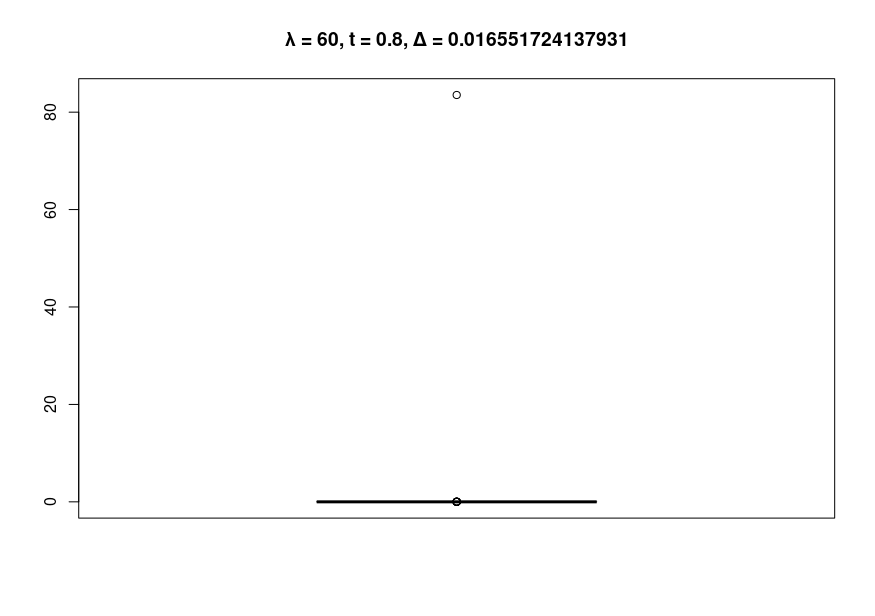
\includegraphics[width=0.47\textwidth]{Images/indiv_vs_glob/qq160.png}
		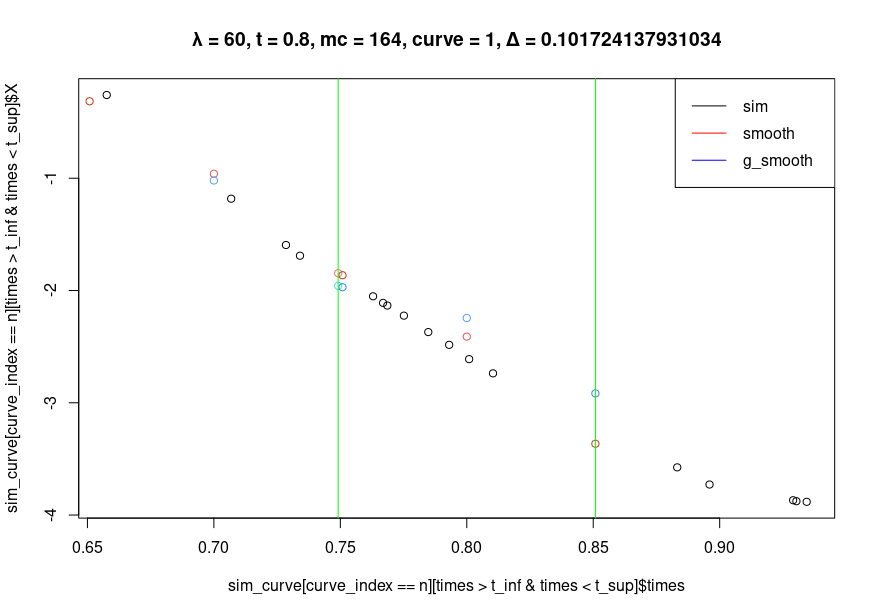
\includegraphics[width=0.47\textwidth]{Images/indiv_vs_glob/lbd60mc164c1.png}
	\end{minipage}

	\begin{minipage}{\linewidth}
		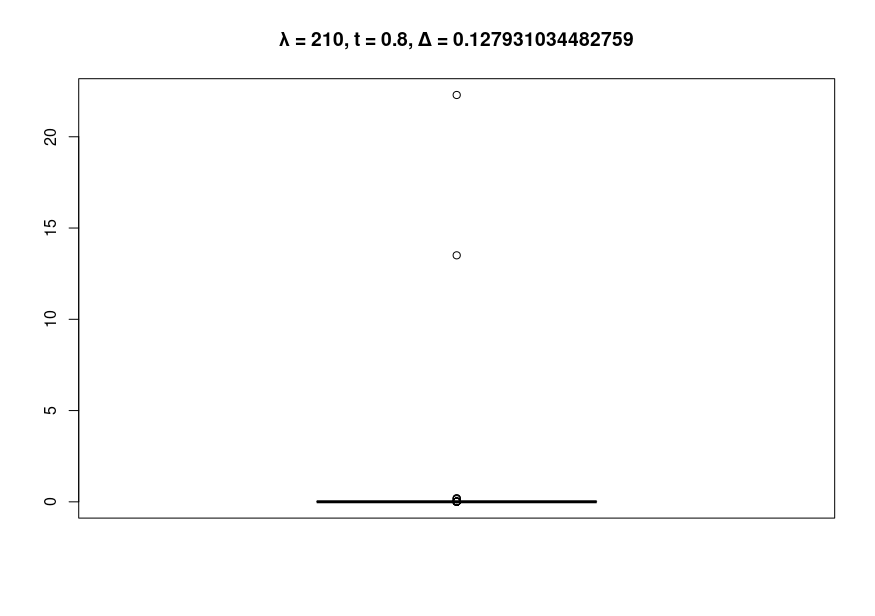
\includegraphics[width=0.47\textwidth]{Images/indiv_vs_glob/qq210.png}
		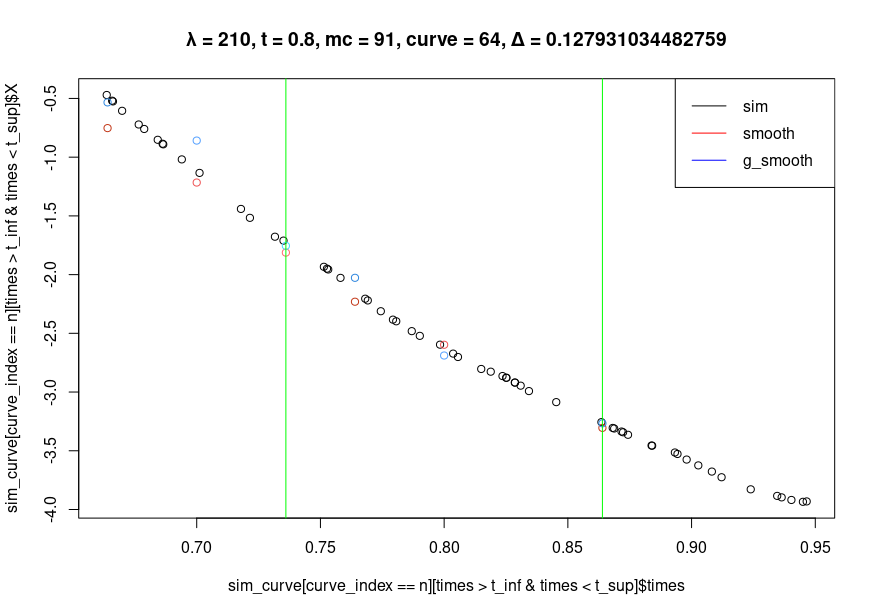
\includegraphics[width=0.47\textwidth]{Images/indiv_vs_glob/lbd210_mc91_c64.png}
	\end{minipage}
	\caption{Distribution des risques et aperçu d'une courbe pour un échantillon de monte carlo extrême sur le risque euclidien.}
	\label{fig:dist_R_eucl_curves}
\end{figure}

\begin{figure}[H]
	\centering
	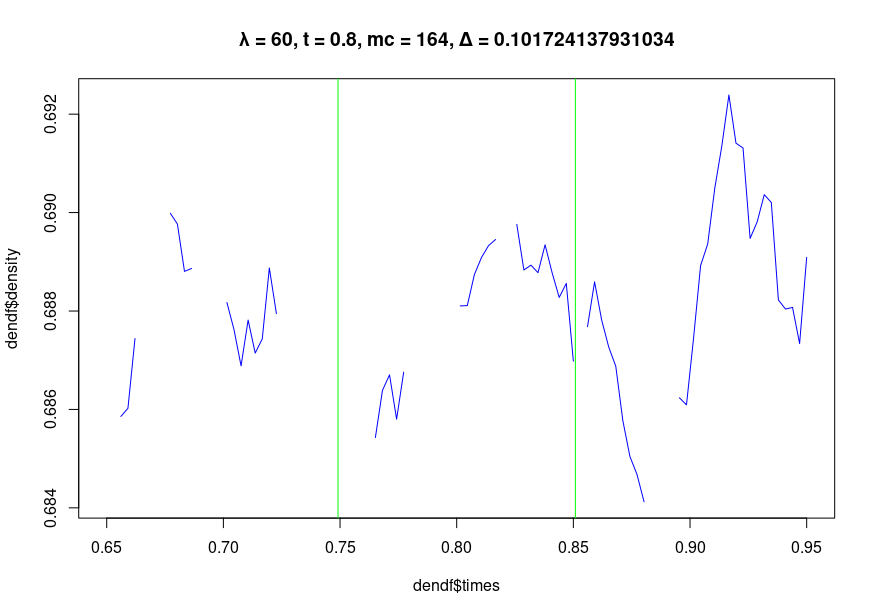
\includegraphics[width=0.7\textwidth]{Images/indiv_vs_glob/Tdensity_lbd60_mc164.png}
	\caption{Densité de points observés sur $[0.65, 0.95]$ pour $\lambda = 60$ sur un échantillon de monte carlo extrême, en un $\Delta$ problématique.}
	\label{fig:den_ex}
\end{figure}


\begin{figure}[H]
	\centering
	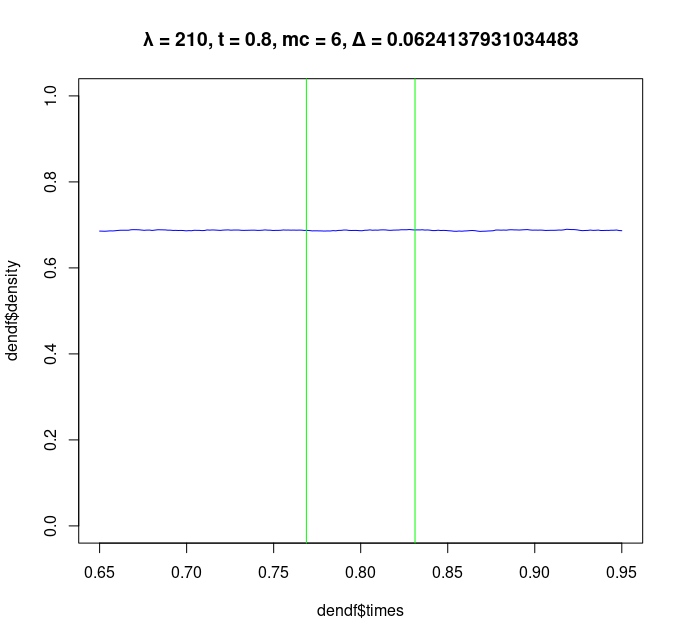
\includegraphics[width=0.4\textwidth]{Images/indiv_vs_glob/worst_210_67_mc6.png}
	\caption{Densité des points observés correspondant à la courbe présentée sur la figure \ref{fig:dist_R_eucl_curves}.}
	\label{fig:den_counterex}
\end{figure}

\begin{figure}[H]
	\centering

	\textbf{avec extrêmes : global}

	\includegraphics[width=0.9\textwidth]{Images/indiv_vs_glob_new/with_xtrm_glob/N200_λ210_t0.8_kernel.jpg}

	\textbf{avec extrêmes : individuel}

	\includegraphics[width=0.9\textwidth]{Images/indiv_vs_glob_new/with_xtrm/N200_λ210_t0.8_kernel.jpg}

	\textbf{sans extrêmes : individuel} (- top 2\%)

	\includegraphics[width=0.9\textwidth]{Images/indiv_vs_glob_new/no_xtrm/N200_λ210_t0.8_kernel.jpg}

	\textbf{sans extrêmes : global} (- top 2\%)

	\includegraphics[width=0.9\textwidth]{Images/indiv_vs_glob_new/no_xtrm_glob/N200_λ210_t0.8_kernel.jpg}
	\caption{Risque Euclidien pour $N=200$, $\lambda=210$ en un point régulier selon la méthode utilisée pour la fenêtre de lissage}
	\label{fig:compare_xtrm}
\end{figure}

\section{Lisser en utilisant une base de fonction sans écraser l'information irrégulière ?}
\label{annexe:lissage_base_fcn}



\subsection{Ondelettes}
\subsubsection{Une brève introduction aux ondelettes}


Les ondelettes proviennent du monde du traîtement du signal. Elles répondent à un problème de représentation des données à la fois dans le domaine temporel et dans le domaine fréquentiel. En effet, la transformée de Fourier nous donne accès aux fréquences présentes dans un signal mais ne nous permet pas de localiser à quel moment sont intervenues les fréquences spécifiques. Le théorème d'indétermination de Heisenberg stipule que l'on ne peut avoir une résolution parfaite à la fois dans le domaine fréquentiel et le domaine temporel, il y a un compromis qui doit être fait. La question devient alors :

\question{
    \smallskip\centering
    Comment représenter une fonction dans le domaine temporel et dans le domaine fréquentiel de façon optimale ? En d'autres termes, quelle résolution temporelle et quelle résolution fréquentielle choisir ?
}

Une première approche proposée en 
% @ todo : compléter date et auteur — STFT
\editorwarn{compléter date} par \editorwarn{compléter auteur}
% @ ————————————
est la transformée de Fourier à court terme (STFT). Celle-ci consiste à regarder la transformée de Fourier d'une fonction sur une fenêtre de taille fixe et à faire glisser cette fenêtre sur la fonction. On obtient ainsi la représentation fréquentielle de la fonction sur un intervalle de temps centré en un point que l'on peut faire varier. 

\bigskip

\begin{minipage}{0.32 \textwidth}
    \begin{figure}[H]
        \centering
        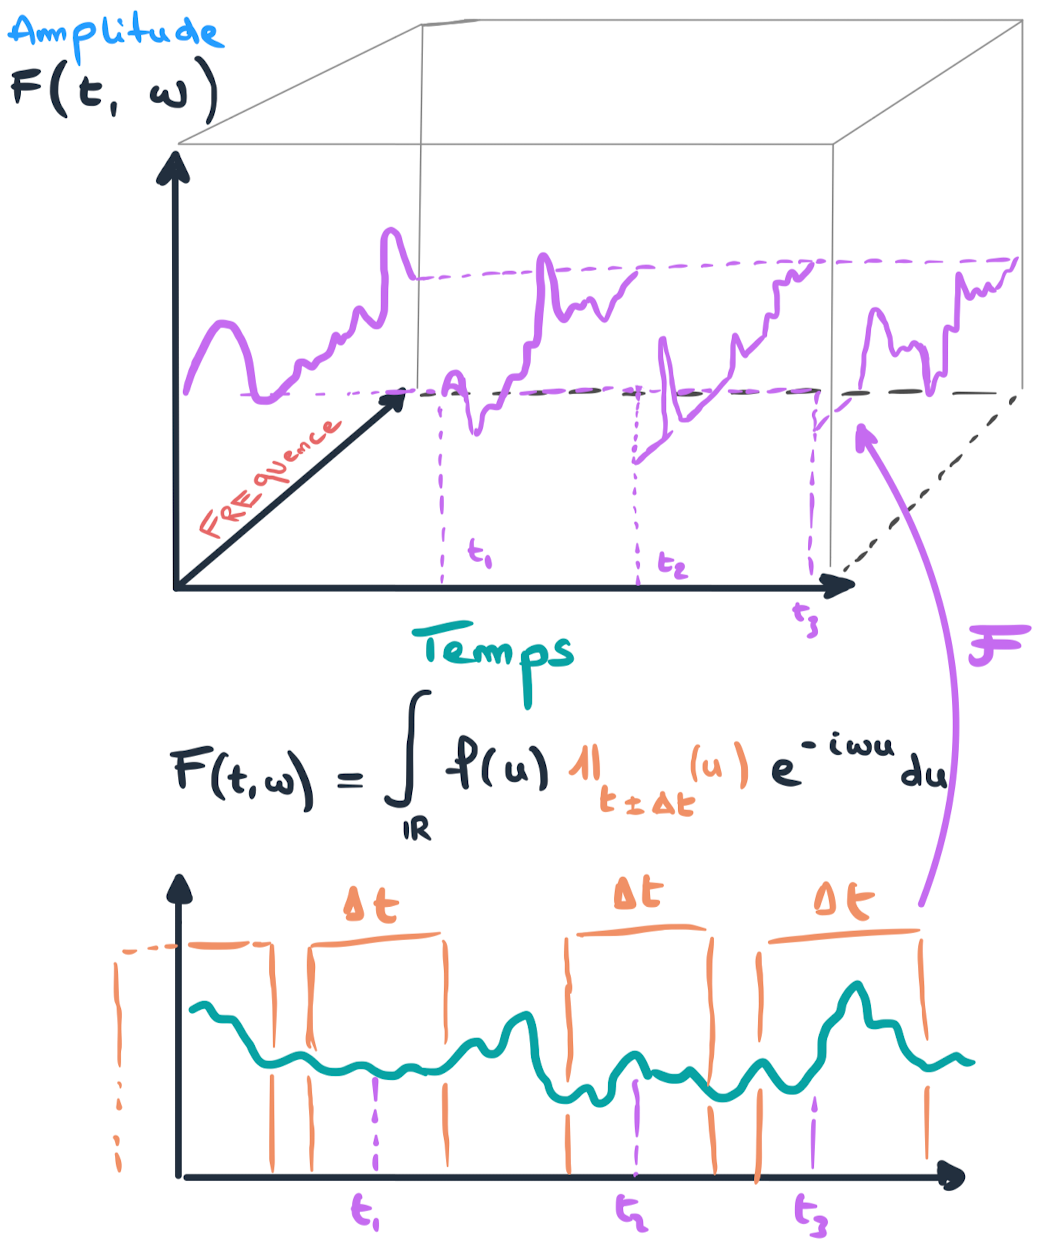
\includegraphics[width=\textwidth]{images/sketches/STFT.png}
        \caption{Transformée de Fourier à court terme d'une fonction}
        \label{fig:STFT}
    \end{figure}
\end{minipage}
\hfill
\begin{minipage}{0.60 \textwidth}
 
    Cependant contrairement à ce que peut suggérer le dessin présenté ici, la résolution fréquentielle n'est pas parfaite. Elle est d'ailleurs dans le cadre de la Transformée de Fourier à court terme constante, que ce soit sur le domaine temporel ou le domaine fréquentiel. La résolution fréquentielle est donc constante quelque soit la fréquence considérée.

    \question{
        \smallskip\centering
        Quel est le problème avec cette approche ?
    }

    le problème ne vient pas du monde mathématique mais plutôt du monde réel : les signaux que l'on observent présentent la caractéristique suivante : Les signaux de basse fréquence ont tendance à s'étendre sur la durée, et les signaux de hautes fréquences ont tendance à être très localisées, sous forme d'impulsion. Il devient alors clair que pour correctement identifier et localiser les fréquences présentes dans un signal, il est judicieux (voire parfois nécessaire) de varier la résolution fréquentielle et temporaire (limitées par le théorème d'indétermination de Heisenberg) en fonction de ce qui est le plus difficile à distinguer. C'est ce que proposent les ondelettes.
    
\end{minipage}

\subsubsection{Théorie de la base ondelettes}

\textbf{Transformée en ondelettes}

Introduisons maintenant de façon plus formelle les ondelettes et regardons leurs propriétés intéressantes dans le cadre du lissage de trajectoires.

on définit la transformée en ondelettes vis à vis de l'ondelette mère $\psi$ d'une fonction $f$ par :

$$F : \begin{array}{ccc}
  \mathds R \times \mathds R_+  &\longrightarrow & \mathds R
    \\
   (t,s) & \longmapsto & \displaystyle\frac 1 { \sqrt{|s|}} \int_{\mathds R} f(\colorize{u}) \psi \left( \frac{\colorize{u}-t}{s} \right) \mathrm d \colorize{u}
\end{array}$$

\brain{on peut remarquer que la formule de la transformée en ondelettes ressemble à une projection : $\displaystyle\frac{\langle f, \psi_{t,s} \rangle_{\mathds L^2}}{|| \psi_{t,s} ||}$. Cela vient en quelque sorte motiver la section suivante}

\textbf{Base d'ondelettes}

$$
\left( \psi_{k,n} : t \mapsto \frac 1 {\sqrt{2^k}} \psi( \frac{t - 2^k n}{2^k} ) \right)_{(k,n) \in \mathds Z^2} \textsf{ est une base } \vcenter{\hbox{$\underset{\| \cdot \|}{\perp}$}} \textsf{ de } \mathds L^2
$$
 
\info{notons que les résolutions sont des puissances de 2, ceci est un détail qui demandera une implémentation particulière dans le cadre des données réelles : il faudra faire attention à ce que le nombre de points que l'on donne dans l'algorithme de transformée rapide en ondelettes soit aussi une puissance de 2.}

\textbf{Propriétés principales des ondelettes}

\smallskip

\begin{itemize}
    \item \textbf{Approximation dans l'espace fréquentiel-temporel} : La transofrmée en ondelettes ( $\mathcal W : f \mapsto \langle f \, | \, \psi_{t,s} \rangle$ ) est une isométrie de $\mathds L^2$. Cela nous permet donc d'affirmer que $|| f - \hat f ||_{\mathds L^2} = || \mathcal W f - \mathcal W \hat f ||_{\mathds L^2}$. Ainsi on peut travailler dans l'espace des ondelettes pour approximer (dans notre cas lisser les trajectoires) des fonctions et contrôler l'approximation directement dans le domaine fréquence-temporel tout en le conservant dans le domaine temporel. \citationrequise
    % @ todo : compléter citation — STFT : talk de Stéphane Mallat

    \item \textbf{Propriété de Fast Decay}
\end{itemize}



\subsubsection{Motivation dans le cadre de l'analyse de données fonctionnelles}

\subsubsection{Effets du lissage à ondelettes sur la régularité locale}

